%  LaTeX support: latex@mdpi.com
%  For support, please attach all files needed for compiling as well as the log file, and specify your operating system, LaTeX version, and LaTeX editor.

%=================================================================
% pandoc conditionals added to preserve backwards compatibility with previous versions of rticles

\documentclass[notspecified,article,submit,moreauthors,pdftex]{Definitions/mdpi}


%% Some pieces required from the pandoc template
\setlist[itemize]{leftmargin=*,labelsep=5.8mm}
\setlist[enumerate]{leftmargin=*,labelsep=4.9mm}


%--------------------
% Class Options:
%--------------------

%---------
% article
%---------
% The default type of manuscript is "article", but can be replaced by:
% abstract, addendum, article, book, bookreview, briefreport, casereport, comment, commentary, communication, conferenceproceedings, correction, conferencereport, entry, expressionofconcern, extendedabstract, datadescriptor, editorial, essay, erratum, hypothesis, interestingimage, obituary, opinion, projectreport, reply, retraction, review, perspective, protocol, shortnote, studyprotocol, systematicreview, supfile, technicalnote, viewpoint, guidelines, registeredreport, tutorial
% supfile = supplementary materials

%----------
% submit
%----------
% The class option "submit" will be changed to "accept" by the Editorial Office when the paper is accepted. This will only make changes to the frontpage (e.g., the logo of the journal will get visible), the headings, and the copyright information. Also, line numbering will be removed. Journal info and pagination for accepted papers will also be assigned by the Editorial Office.

%------------------
% moreauthors
%------------------
% If there is only one author the class option oneauthor should be used. Otherwise use the class option moreauthors.

%---------
% pdftex
%---------
% The option pdftex is for use with pdfLaTeX. Remove "pdftex" for (1) compiling with LaTeX & dvi2pdf (if eps figures are used) or for (2) compiling with XeLaTeX.

%=================================================================
% MDPI internal commands - do not modify
\firstpage{1}
\makeatletter
\setcounter{page}{\@firstpage}
\makeatother
\pubvolume{1}
\issuenum{1}
\articlenumber{0}
\pubyear{2023}
\copyrightyear{2023}
%\externaleditor{Academic Editor: Firstname Lastname}
\datereceived{ }
\daterevised{ } % Comment out if no revised date
\dateaccepted{ }
\datepublished{ }
%\datecorrected{} % For corrected papers: "Corrected: XXX" date in the original paper.
%\dateretracted{} % For corrected papers: "Retracted: XXX" date in the original paper.
\hreflink{https://doi.org/} % If needed use \linebreak
%\doinum{}
%\pdfoutput=1 % Uncommented for upload to arXiv.org

%=================================================================
% Add packages and commands here. The following packages are loaded in our class file: fontenc, inputenc, calc, indentfirst, fancyhdr, graphicx, epstopdf, lastpage, ifthen, float, amsmath, amssymb, lineno, setspace, enumitem, mathpazo, booktabs, titlesec, etoolbox, tabto, xcolor, colortbl, soul, multirow, microtype, tikz, totcount, changepage, attrib, upgreek, array, tabularx, pbox, ragged2e, tocloft, marginnote, marginfix, enotez, amsthm, natbib, hyperref, cleveref, scrextend, url, geometry, newfloat, caption, draftwatermark, seqsplit
% cleveref: load \crefname definitions after \begin{document}

%=================================================================
% Please use the following mathematics environments: Theorem, Lemma, Corollary, Proposition, Characterization, Property, Problem, Example, ExamplesandDefinitions, Hypothesis, Remark, Definition, Notation, Assumption
%% For proofs, please use the proof environment (the amsthm package is loaded by the MDPI class).

%=================================================================
% Full title of the paper (Capitalized)
\Title{Análisis Exploratorio de los Logs del Aula Virtual: Grupo E}

% MDPI internal command: Title for citation in the left column
\TitleCitation{Análisis Exploratorio de los Logs del Aula Virtual: Grupo
E}

% Author Orchid ID: enter ID or remove command
%\newcommand{\orcidauthorA}{0000-0000-0000-000X} % Add \orcidA{} behind the author's name
%\newcommand{\orcidauthorB}{0000-0000-0000-000X} % Add \orcidB{} behind the author's name


% Authors, for the paper (add full first names)
\Author{(Eva Gamón)$^{1}$, (Marina Moros)$^{1}$, (Irene
Pérez)$^{1}$, (Maria Martínez)$^{1}$, (Tomas Payás)$^{1}$}


%\longauthorlist{yes}


% MDPI internal command: Authors, for metadata in PDF
\AuthorNames{(Eva Gamón), (Marina Moros), (Irene Pérez), (Maria
Martínez), (Tomas Payás)}

% MDPI internal command: Authors, for citation in the left column
%\AuthorCitation{Lastname, F.; Lastname, F.; Lastname, F.}
% If this is a Chicago style journal: Lastname, Firstname, Firstname Lastname, and Firstname Lastname.
\AuthorCitation{(Apellidos Alumnos)}

% Affiliations / Addresses (Add [1] after \address if there is only one affiliation.)
\address{%
$^{1}$ \quad Grado en Ciencia de Datos Universidad de Valencia,
España; (email)\citet{alumni.uv.es}\\
}

% Contact information of the corresponding author
\corres{Correspondence: }

% Current address and/or shared authorship








% The commands \thirdnote{} till \eighthnote{} are available for further notes

% Simple summary
\simplesumm{Este trabajo analiza el comportamiento de los estudiantes
mediante los registros de actividad del Aula Virtual.}

%\conference{} % An extended version of a conference paper

% Abstract (Do not insert blank lines, i.e. \\)
\abstract{Este trabajo analiza el comportamiento de los estudiantes
mediante los registros de actividad del Aula Virtual, aplicando un
Análisis Exploratorio de Tatamiento de Datos (TD) con R y Tidyverse. El
objetivo es extraer patrones de interacción y transformar datos brutos
en información útil.}


% Keywords
\keyword{Análisis exploratorio; R; Logs; Aula Virtual; Tidyverse.}

% The fields PACS, MSC, and JEL may be left empty or commented out if not applicable
%\PACS{J0101}
%\MSC{}
%\JEL{}

%%%%%%%%%%%%%%%%%%%%%%%%%%%%%%%%%%%%%%%%%%
% Only for the journal Diversity
%\LSID{\url{http://}}

%%%%%%%%%%%%%%%%%%%%%%%%%%%%%%%%%%%%%%%%%%
% Only for the journal Applied Sciences

%%%%%%%%%%%%%%%%%%%%%%%%%%%%%%%%%%%%%%%%%%

%%%%%%%%%%%%%%%%%%%%%%%%%%%%%%%%%%%%%%%%%%
% Only for the journal Data



%%%%%%%%%%%%%%%%%%%%%%%%%%%%%%%%%%%%%%%%%%
% Only for the journal Toxins


%%%%%%%%%%%%%%%%%%%%%%%%%%%%%%%%%%%%%%%%%%
% Only for the journal Encyclopedia


%%%%%%%%%%%%%%%%%%%%%%%%%%%%%%%%%%%%%%%%%%
% Only for the journal Advances in Respiratory Medicine
%\addhighlights{yes}
%\renewcommand{\addhighlights}{%

%\noindent This is an obligatory section in “Advances in Respiratory Medicine”, whose goal is to increase the discoverability and readability of the article via search engines and other scholars. Highlights should not be a copy of the abstract, but a simple text allowing the reader to quickly and simplified find out what the article is about and what can be cited from it. Each of these parts should be devoted up to 2~bullet points.\vspace{3pt}\\
%\textbf{What are the main findings?}
% \begin{itemize}[labelsep=2.5mm,topsep=-3pt]
% \item First bullet.
% \item Second bullet.
% \end{itemize}\vspace{3pt}
%\textbf{What is the implication of the main finding?}
% \begin{itemize}[labelsep=2.5mm,topsep=-3pt]
% \item First bullet.
% \item Second bullet.
% \end{itemize}
%}


%%%%%%%%%%%%%%%%%%%%%%%%%%%%%%%%%%%%%%%%%%

% Pandoc syntax highlighting
\usepackage{color}
\usepackage{fancyvrb}
\newcommand{\VerbBar}{|}
\newcommand{\VERB}{\Verb[commandchars=\\\{\}]}
\DefineVerbatimEnvironment{Highlighting}{Verbatim}{commandchars=\\\{\}}
% Add ',fontsize=\small' for more characters per line
\usepackage{framed}
\definecolor{shadecolor}{RGB}{248,248,248}
\newenvironment{Shaded}{\begin{snugshade}}{\end{snugshade}}
\newcommand{\AlertTok}[1]{\textcolor[rgb]{0.94,0.16,0.16}{#1}}
\newcommand{\AnnotationTok}[1]{\textcolor[rgb]{0.56,0.35,0.01}{\textbf{\textit{#1}}}}
\newcommand{\AttributeTok}[1]{\textcolor[rgb]{0.13,0.29,0.53}{#1}}
\newcommand{\BaseNTok}[1]{\textcolor[rgb]{0.00,0.00,0.81}{#1}}
\newcommand{\BuiltInTok}[1]{#1}
\newcommand{\CharTok}[1]{\textcolor[rgb]{0.31,0.60,0.02}{#1}}
\newcommand{\CommentTok}[1]{\textcolor[rgb]{0.56,0.35,0.01}{\textit{#1}}}
\newcommand{\CommentVarTok}[1]{\textcolor[rgb]{0.56,0.35,0.01}{\textbf{\textit{#1}}}}
\newcommand{\ConstantTok}[1]{\textcolor[rgb]{0.56,0.35,0.01}{#1}}
\newcommand{\ControlFlowTok}[1]{\textcolor[rgb]{0.13,0.29,0.53}{\textbf{#1}}}
\newcommand{\DataTypeTok}[1]{\textcolor[rgb]{0.13,0.29,0.53}{#1}}
\newcommand{\DecValTok}[1]{\textcolor[rgb]{0.00,0.00,0.81}{#1}}
\newcommand{\DocumentationTok}[1]{\textcolor[rgb]{0.56,0.35,0.01}{\textbf{\textit{#1}}}}
\newcommand{\ErrorTok}[1]{\textcolor[rgb]{0.64,0.00,0.00}{\textbf{#1}}}
\newcommand{\ExtensionTok}[1]{#1}
\newcommand{\FloatTok}[1]{\textcolor[rgb]{0.00,0.00,0.81}{#1}}
\newcommand{\FunctionTok}[1]{\textcolor[rgb]{0.13,0.29,0.53}{\textbf{#1}}}
\newcommand{\ImportTok}[1]{#1}
\newcommand{\InformationTok}[1]{\textcolor[rgb]{0.56,0.35,0.01}{\textbf{\textit{#1}}}}
\newcommand{\KeywordTok}[1]{\textcolor[rgb]{0.13,0.29,0.53}{\textbf{#1}}}
\newcommand{\NormalTok}[1]{#1}
\newcommand{\OperatorTok}[1]{\textcolor[rgb]{0.81,0.36,0.00}{\textbf{#1}}}
\newcommand{\OtherTok}[1]{\textcolor[rgb]{0.56,0.35,0.01}{#1}}
\newcommand{\PreprocessorTok}[1]{\textcolor[rgb]{0.56,0.35,0.01}{\textit{#1}}}
\newcommand{\RegionMarkerTok}[1]{#1}
\newcommand{\SpecialCharTok}[1]{\textcolor[rgb]{0.81,0.36,0.00}{\textbf{#1}}}
\newcommand{\SpecialStringTok}[1]{\textcolor[rgb]{0.31,0.60,0.02}{#1}}
\newcommand{\StringTok}[1]{\textcolor[rgb]{0.31,0.60,0.02}{#1}}
\newcommand{\VariableTok}[1]{\textcolor[rgb]{0.00,0.00,0.00}{#1}}
\newcommand{\VerbatimStringTok}[1]{\textcolor[rgb]{0.31,0.60,0.02}{#1}}
\newcommand{\WarningTok}[1]{\textcolor[rgb]{0.56,0.35,0.01}{\textbf{\textit{#1}}}}

% tightlist command for lists without linebreak
\providecommand{\tightlist}{%
  \setlength{\itemsep}{0pt}\setlength{\parskip}{0pt}}

% From pandoc table feature
\usepackage{longtable,booktabs,array}
\usepackage{calc} % for calculating minipage widths
% Correct order of tables after \paragraph or \subparagraph
\usepackage{etoolbox}
\makeatletter
\patchcmd\longtable{\par}{\if@noskipsec\mbox{}\fi\par}{}{}
\makeatother
% Allow footnotes in longtable head/foot
\IfFileExists{footnotehyper.sty}{\usepackage{footnotehyper}}{\usepackage{footnote}}
\makesavenoteenv{longtable}


\newcommand{\pandocbounded}[1]{#1}
\usepackage{longtable}
\usepackage{booktabs}
\usepackage{array}
\usepackage{multirow}
\usepackage{wrapfig}
\usepackage{float}
\usepackage{colortbl}
\usepackage{pdflscape}
\usepackage{tabu}
\usepackage{threeparttable}
\usepackage{threeparttablex}
\usepackage[normalem]{ulem}
\usepackage{makecell}
\usepackage{xcolor}

\begin{document}



%%%%%%%%%%%%%%%%%%%%%%%%%%%%%%%%%%%%%%%%%%

\section{Introducción}\label{introducciuxf3n}

En la era digital actual, las plataformas de aprendizaje virtual como el
Aula Virtual se han convertido en el núcleo operativo de la educación
universitaria. Estas plataformas no solo facilitan el acceso a los
materiales y la entrega de tareas, sino que también generan un rastro
digital exhaustivo de las interacciones de los usuarios mediante
archivos de registro o \emph{logs}.

Este proyecto tiene como objetivo principal poner en práctica los
conocimientos de Análisis Exploratorio de Datos adquiridos durante la
asignatura de ``Tratamiento de los Datos'' del Grado en Ciencia de
Datos. Para llevar a cabo este análisis, trabajaremos con un conjunto de
datos real proporcionado por el profesor de la asignatura: los
\emph{logs} anonimizados del Aula Virtual de esta misma asignatura,
correspondientes al curso académico 2024-2025.

Mediante el uso del lenguaje de programación R y, en particular, del
ecosistema \emph{tidyverse} (con librerías como \texttt{dplyr},
\texttt{tidyr} y \texttt{ggplot2}), realizaremos un proceso completo de
importación, limpieza, adecuación y visualización de los datos. El
propósito es extraer patrones de comportamiento subyacentes que nos
permitan entender cómo interactúan los alumnos con la plataforma.

A lo largo de este documento, plantearemos y daremos respuesta a una
serie de preguntas clave, tales como la distribución temporal de las
conexiones, los recursos más consultados o los picos de actividad. De
este modo, buscamos transformar un conjunto de datos en bruto en
información útil y visualmente interpretable.

\section{Material y métodos}\label{material-y-muxe9todos}

En esta fase se ha llevado a cabo la importación de los datos en bruto
para convertirlos en un conjunto de datos técnicamente correcto. Para
ello, se han renombrado las variables conflictivas y se ha convertido la
variable temporal a un formato de fecha válido utilizando la librería
lubridate. Como se puede observar en la Tabla 1, los datos han sido
importados y preprocesados correctamente para su posterior análisis
exploratorio.

\begin{Shaded}
\begin{Highlighting}[]
\CommentTok{\# Importación de los datos}
\NormalTok{archivo\_datos }\OtherTok{\textless{}{-}} \StringTok{"data/logs\_moodle\_anon.csv"}
\NormalTok{datos\_brutos }\OtherTok{\textless{}{-}} \FunctionTok{read.csv}\NormalTok{(archivo\_datos, }\AttributeTok{fileEncoding =} \StringTok{"UTF{-}8"}\NormalTok{)}

\CommentTok{\# Preparación y tratamiento de fechas }
\NormalTok{datos\_logs }\OtherTok{\textless{}{-}}\NormalTok{ datos\_brutos }\SpecialCharTok{\%\textgreater{}\%}
  \CommentTok{\# Renombramos columnas (sin espacios)}
  \FunctionTok{rename}\NormalTok{(}
    \AttributeTok{Usuario =}\NormalTok{ Nombre.completo.del.usuario,}
    \AttributeTok{Contexto =}\NormalTok{ Contexto.del.evento,}
    \AttributeTok{Evento =}\NormalTok{ Nombre.evento}
\NormalTok{  ) }\SpecialCharTok{\%\textgreater{}\%}
  \CommentTok{\# Tratamiento de fecha con lubridate}
  \FunctionTok{mutate}\NormalTok{(}
    \AttributeTok{Fecha\_aux =} \FunctionTok{dmy\_hms}\NormalTok{(Hora),}
    \AttributeTok{Fecha\_texto =} \FunctionTok{format}\NormalTok{(Fecha\_aux, }\StringTok{"\%d/\%m/\%Y"}\NormalTok{)}
\NormalTok{  )}

\CommentTok{\# Comprobación }
\FunctionTok{kable}\NormalTok{(}\FunctionTok{head}\NormalTok{(datos\_logs, }\DecValTok{5}\NormalTok{), }\AttributeTok{caption =} \StringTok{"Primeros registros de la base de datos"}\NormalTok{) }\SpecialCharTok{\%\textgreater{}\%}
  \FunctionTok{kable\_styling}\NormalTok{(}\AttributeTok{latex\_options =} \StringTok{"scale\_down"}\NormalTok{)}
\end{Highlighting}
\end{Shaded}

\begin{verbatim}
## Warning in styling_latex_scale(out, table_info, "down"): Longtable cannot be
## resized.
\end{verbatim}

\begin{longtable}[t]{lllllllllll}
\caption{\label{tab:unnamed-chunk-1}Primeros registros de la base de datos}\\
\toprule
Hora & Usuario & Usuario.afectado & Contexto & Componente & Evento & Descripción & Origen & Dirección.IP & Fecha\_aux & Fecha\_texto\\
\midrule
3/03/26, 10:59:04 & U0072 & NA & Curso: 2024-25 Tractament de les dades Gr.A-T (36423) & Registros & Informe de registro visualizado & The user with id '22872' viewed the log report for the course with id '85837'. & web & 2001:720:1014:88:0:0:a:6b7 & 2026-03-03 10:59:04 & 03/03/2026\\
3/03/26, 10:58:57 & U0072 & NA & Curso: 2024-25 Tractament de les dades Gr.A-T (36423) & Registros & Informe de registro visualizado & The user with id '22872' viewed the log report for the course with id '85837'. & web & 2001:720:1014:88:0:0:a:6b7 & 2026-03-03 10:58:57 & 03/03/2026\\
3/03/26, 10:58:30 & U0072 & NA & Curso: 2024-25 Tractament de les dades Gr.A-T (36423) & Actividad del curso & Informe de actividad visto & The user with id '22872' viewed the outline activity report for the course with id '85837'. & web & 2001:720:1014:88:0:0:a:6b7 & 2026-03-03 10:58:30 & 03/03/2026\\
3/03/26, 10:57:28 & U0072 & NA & Curso: 2024-25 Tractament de les dades Gr.A-T (36423) & Actividad del curso & Informe de actividad visto & The user with id '22872' viewed the outline activity report for the course with id '85837'. & web & 2001:720:1014:88:0:0:a:6b7 & 2026-03-03 10:57:28 & 03/03/2026\\
3/03/26, 10:57:09 & U0072 & NA & Curso: 2024-25 Tractament de les dades Gr.A-T (36423) & Sistema & Curso visto & The user with id '22872' viewed the course with id '85837'. & web & 2001:720:1014:88:0:0:a:6b7 & 2026-03-03 10:57:09 & 03/03/2026\\
\bottomrule
\end{longtable}

\section{Figuras y tablas numeradas y
referenciadas.}\label{figuras-y-tablas-numeradas-y-referenciadas.}

En este proyecto utilizaremos figuras y tablas para poder interpretar de
una manera más clara y visual la información obtenida a partir de los
datos analizados.

\subsection{Tablas:}\label{tablas}

Queremos mostrar el número de veces que aparece cada tipo de evento,
identificando así las acciones que los usuarios realizan de manera más
habitual.

\begin{longtable}[]{@{}lr@{}}
\caption{Frecuencia de eventos registrados}\tabularnewline
\toprule\noalign{}
Evento & Cantidad \\
\midrule\noalign{}
\endfirsthead
\toprule\noalign{}
Evento & Cantidad \\
\midrule\noalign{}
\endhead
\bottomrule\noalign{}
\endlastfoot
Módulo de curso visto & 23535 \\
Curso visto & 20430 \\
Usuario calificado & 12846 \\
Se ha visualizado el estado de la entrega. & 9388 \\
Intento de cuestionario visualizado & 3877 \\
Intento de cuestionario actualizado & 3676 \\
Pregunta creada & 3395 \\
Informe de notas de usuario visto & 2771 \\
Informe de sesión visto & 2680 \\
Intento de cuestionario guardado automáticamente & 2618 \\
Evento de calendario actualizado & 1558 \\
Formulario de entrega visto. & 1499 \\
Elemento de calificación actualizado & 1345 \\
Se ha enviado una entrega & 1319 \\
Un fichero ha sido subido. & 1319 \\
Entrega creada. & 1215 \\
Calificación borrada & 1153 \\
Lista de usuarios vista & 1135 \\
Resumen del intento de cuestionario visualizado & 1032 \\
Directorio descargado en formato Zip & 986 \\
Ha comenzado el intento & 965 \\
Intento enviado & 926 \\
Perfil de usuario visto & 885 \\
Asistencia confirmada por el alumno & 884 \\
Retroalimentación vista & 805 \\
Formulario de calificaciones visto & 793 \\
Se ha calificado el envío. & 659 \\
Módulo de curso actualizado & 657 \\
Respuestas enviadas & 506 \\
Visualización de las Calificaciones & 457 \\
Informe del calificador visto & 309 \\
Miembro del grupo añadido & 308 \\
Informe de cuestionario visto & 294 \\
Reporte de Respuestas Individuales visto & 253 \\
Creada ranura & 245 \\
Categoría de preguntas creada & 176 \\
Envío actualizado. & 158 \\
Tema visto & 155 \\
Pregunta borrada & 148 \\
Informe de calificación de vista simple visto. & 146 \\
Reporte de Todas las Respuestas visto & 143 \\
Rol asignado & 138 \\
Usuario matriculado en el curso & 138 \\
Ranura eliminada & 131 \\
Evento de calendario creado & 112 \\
Página de edición del cuestionario visitada & 104 \\
Elemento de calificación creado & 93 \\
Intento de cuestionario recalificado & 92 \\
Categoría de preguntas visualizada & 88 \\
Informe usuario del curso visto & 63 \\
Grupo creado & 56 \\
Grupo asignado al agrupamiento & 55 \\
Tiempo límite del cuestionario excedido & 55 \\
Todos los envíos se están descargando. & 55 \\
Un texto en línea ha sido subido. & 54 \\
Sesión actualizada & 50 \\
Sección de curso actualizado & 48 \\
Borrar la confirmación de envío visualizada. & 42 \\
Elemento borrado & 41 \\
Elemento creado & 41 \\
Módulo de curso eliminado & 41 \\
Intento abandonado & 40 \\
Módulo de curso creado & 39 \\
El estado de la entrega se ha actualizado. & 37 \\
Envío eliminado & 37 \\
Pregunta movida & 37 \\
Intento del cuestionario revisado & 35 \\
El usuario ha aceptado la declaración del envío. & 30 \\
Comentario creado & 23 \\
Algún contenido ha sido publicado. & 22 \\
Espacio movido & 19 \\
Pregunta visualizada & 19 \\
Preguntas importadas & 19 \\
Sección del curso creada & 19 \\
Tema creado & 19 \\
Evento de calendario borrado & 18 \\
Instancia del módulo del curso visualizada & 18 \\
Calificación exportada & 17 \\
Vista previa del intento iniciada & 17 \\
Elemento de calificación eliminado & 15 \\
Asistencia confirmada & 14 \\
Informe de resumen de notas visto & 12 \\
Sección vista & 11 \\
Cuestionario re-paginado & 9 \\
Informe de registro visualizado & 9 \\
Mezcla aleatoria de secciones actualizada & 9 \\
Carpeta actualizada & 7 \\
Agrupamiento creado & 6 \\
Calificación XLS exportada & 5 \\
Sesión añadida & 4 \\
Agrupamiento eliminado & 3 \\
Instancia de inscripción creada & 3 \\
Miembro del grupo eliminado & 3 \\
Agrupamiento actualizado & 2 \\
Curso buscado & 2 \\
Curso restaurado & 2 \\
Informe de actividad visto & 2 \\
Mensaje creado & 2 \\
Preguntas exportadas & 2 \\
Sesión eliminada & 2 \\
Categoría de preguntas actualizada & 1 \\
Copia de curso creada & 1 \\
Curso creado & 1 \\
Grupo eliminado & 1 \\
Informe de participación visto & 1 \\
Informe del usuario visualizado & 1 \\
Mensaje actualizado & 1 \\
Rol sin asignar & 1 \\
Sección de curso eliminada & 1 \\
Todas las Respuestas guardadas como texto & 1 \\
Usuario desmatriculado del curso & 1 \\
\end{longtable}

En la Tabla \ref{fig:tabla-eventos} vemos los eventos más habituales
entre los usuarios.

\subsection{Figura:}\label{figura}

Vamos a crear un diagrama de barras que nos permite visualizar cuáles
son los tipos de eventos más frecuentes

En la Figura \ref{fig:figura-eventos} podemos observar cuáles son los
eventos más frecuentes entre los usuarios.

\begin{figure}

{\centering 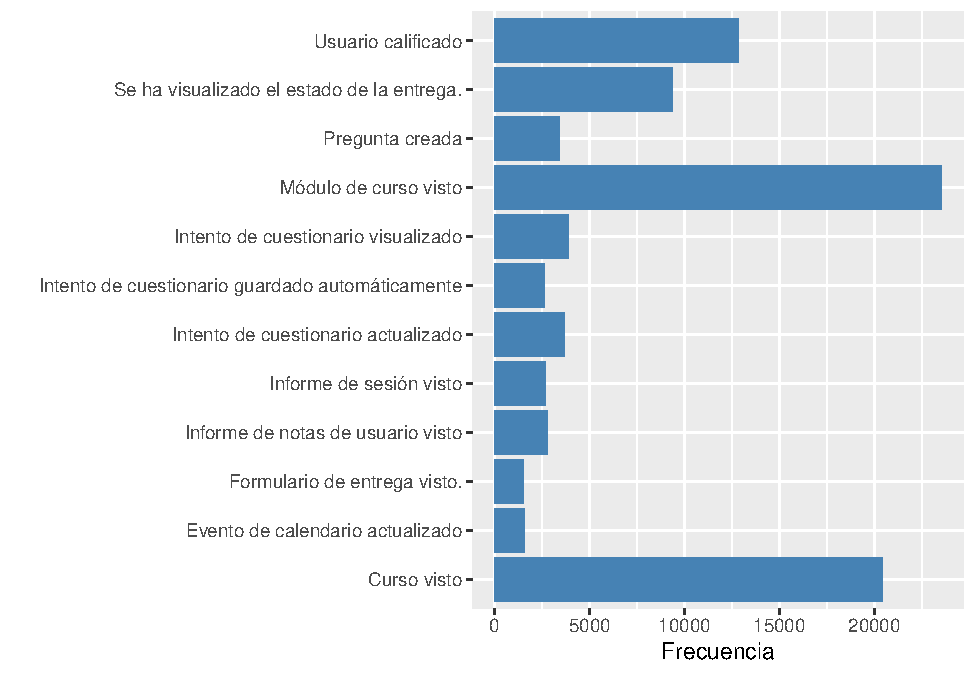
\includegraphics[width=1\linewidth]{ProyectoTD2026_files/figure-latex/figura-eventos-1} 

}

\caption{Diagrama de barras de los eventos más frecuentes}\label{fig:figura-eventos}
\end{figure}

\section{Exploración y
Visualización}\label{exploraciuxf3n-y-visualizaciuxf3n}

Una vez que los datos han sido organizados en una estructura adecuada y
se ha verificado su consistencia,comienza una fase clave del análisis:
la exploración. En este punto, el objetivo no es todavia confirmar
conclusiones, sino observar,comparar y cuestionar la información
otorgada. A partir del conjunto de datos dado nos surgen varias
hipótesis provisionales sobre posibles tendencias,relaciones o
comportamientos. En el siguiente apartado se expondrán dichas preguntas
claves para la exploración de los datos

1.¿En que hora existe una mayor actividad por parte de los alumnos ?

2.¿Se generan picos antes de la entrega de un proyecto?

3.¿Qué usuarios son más activos (mayor número de eventos)?

4.¿Existen usuarios con comportamiento atípico (muy alta o muy baja
actividad)?

5.¿Existe relación entre el dispositivo empleado y la actividad
realizada?

6.¿Que actividades o recursos generan más interacciones?

7.¿Hay registros realizados en horas ``extrañas'' (ej. 4:00 AM)? ¿Son
usuarios aislados o un patrón común en época de exámenes?

8.¿Se detectan múltiples IPs para un mismo usuario en un corto periodo
de tiempo?

9.¿Hay eventos de error o acciones fallidas recurrentes en los logs?

10.¿Existe alguna evolución en la actividad de un mismo usuario a lo
largo del año (de menos a más o de más a menos)? ¿A que puede deberse
esto?

11.¿Hay una diferencia notoria entre las actividades registradas en dias
lectivos y las registradas los fines de semana?

12.¿Que franjas horarias muestran una mayor concentración de usuarios al
mismo tiempo?

13.¿Cuál es la proporción entre el número de actividades pasivas
(entrar, ver) y las activas (entregar, editar)?

14.¿Existen usuarios que solo acceden en momentos muy concretos? (Ej.
previos a entrega o a exámenes)

15.¿En horario lectivo se detecta menor actividad desde el móvil o es
indiferente?

16.¿Hay más actividad en días laborales o en fin de semana? ¿Varia esta
proporción en momentos concretos? (Ej. época de exámenes)

\subsection{Análisis univariante}\label{anuxe1lisis-univariante}

En nuestro data frame observamos la predominancia de variables de tipo
string o factor, de modo que las tablas realizadas no mostrarán
estadísticos descriptivos. En este caso, se centraran en frecuencias,
porcentajes y descripciones.

\begin{longtable}[]{@{}
  >{\raggedright\arraybackslash}p{(\linewidth - 4\tabcolsep) * \real{0.1857}}
  >{\raggedright\arraybackslash}p{(\linewidth - 4\tabcolsep) * \real{0.1000}}
  >{\raggedright\arraybackslash}p{(\linewidth - 4\tabcolsep) * \real{0.7143}}@{}}
\caption{Descripción de las variables}\tabularnewline
\toprule\noalign{}
\begin{minipage}[b]{\linewidth}\raggedright
Variable
\end{minipage} & \begin{minipage}[b]{\linewidth}\raggedright
Tipo
\end{minipage} & \begin{minipage}[b]{\linewidth}\raggedright
Descripción
\end{minipage} \\
\midrule\noalign{}
\endfirsthead
\toprule\noalign{}
\begin{minipage}[b]{\linewidth}\raggedright
Variable
\end{minipage} & \begin{minipage}[b]{\linewidth}\raggedright
Tipo
\end{minipage} & \begin{minipage}[b]{\linewidth}\raggedright
Descripción
\end{minipage} \\
\midrule\noalign{}
\endhead
\bottomrule\noalign{}
\endlastfoot
Usuario & Factor & Identificador anónimo del alumno \\
Contexto & String & Nombre del curso o tarea donde ocurre la acción \\
Componente & Factor & Módulo del sistema (Tarea, Cuestionario,
Sistema) \\
Evento & Factor & Acción específica realizada por el usuario \\
Dirección.IP & String & Dirección desde la que se conecta \\
hora\_dia & Entero & Hora del día en formato 24h \\
\end{longtable}

Como se puede observar en la Tabla \ref{tab:tabla-variables}, existe una
predominancia de variables de tipo string o factor.

\begin{longtable}[]{@{}lr@{}}
\caption{Análisis de valores faltantes por variable}\tabularnewline
\toprule\noalign{}
Variable & ValoresFaltantes \\
\midrule\noalign{}
\endfirsthead
\toprule\noalign{}
Variable & ValoresFaltantes \\
\midrule\noalign{}
\endhead
\bottomrule\noalign{}
\endlastfoot
Hora & 0 \\
Usuario & 0 \\
Usuario.afectado & 69346 \\
Contexto & 0 \\
Componente & 0 \\
Evento & 0 \\
Descripción & 0 \\
Origen & 0 \\
Dirección.IP & 2857 \\
Fecha\_aux & 0 \\
Fecha\_texto & 0 \\
\end{longtable}

A partir de los datos obtenidos en la Tabla \ref{tab:analisis-nas} se
puede afirmar que el conjunto de datos es robusto, es decir, existe un
escaso porcentaje de valores faltantes en las variables analizadas.

Por otro lado, la existencia de valores nulos en variables como
``Usuario.afectado'' no deben interpretarse como errores, ya que existen
múltiples acciones que son individuales y no requieren la implicación de
un segundo usuario. Por tanto, el data set es considerado de alta
calidad.

Una vez confirmada la integridad del data frame obtenido y analizada la
naturaleza de las variables que lo componen procedemos a realizar una
análisis descriptivo, en el cual trataremos de identificar los patrones
de coportamiento de los estudiantes. Por ende ,analizaremos los picos de
actividad y los materiales consultados con mayor frecuencia.

\section{Análisis de la distribución
horaria}\label{anuxe1lisis-de-la-distribuciuxf3n-horaria}

Para determinar la franja horaria en la que existe una mayor actividad
por parte del alumnado, analizaremos la distribución.Esta nos permite
comprender y analizar el comportamiento de los estudiantes.

En este caso contemplaremos tanto la forma de la distribución(Gráfica
1), como el número de interacciones por franjas horarias(Gráfica 2)

\begin{figure}

{\centering 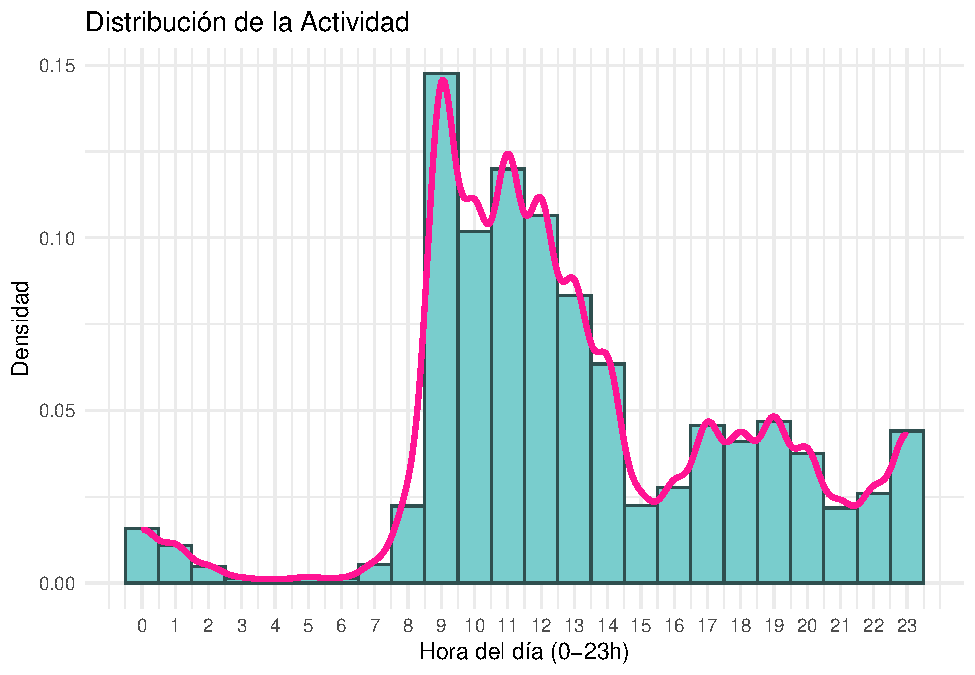
\includegraphics[width=1\linewidth]{ProyectoTD2026_files/figure-latex/grafico-densidad-1} 

}

\caption{Análisis densidad}\label{fig:grafico-densidad}
\end{figure}

\textless\textless\textless\textless\textless\textless\textless{} HEAD

\begin{figure}

{\centering 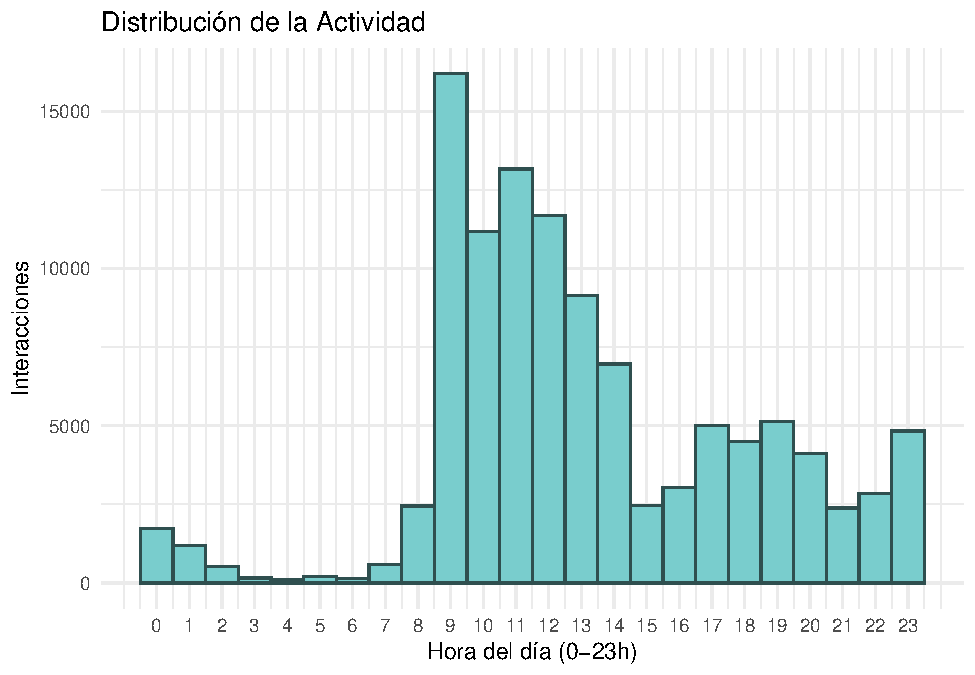
\includegraphics[width=1\linewidth]{ProyectoTD2026_files/figure-latex/grafico-horas-1} 

}

\caption{Distribución de la actividad de los usuarios por hora del día}\label{fig:grafico-horas}
\end{figure}

Como se puede observar en las Figura \ref{fig:grafico-horas},el uso de
la plataforma presenta una gran variación a lo largo del día. La mayor
parte de la actividad se concentra durante la mañana, alcanzando su pico
máximo durante las 9:00 horas, podemos observar que en ese instante se
registran más de 16.000 eventos. Este comportamiento es coherente con el
horario lectivo.

Por otro lado, podemos apreciar como la caída de la actividad durante
las horas centrales del mediodía (14:00 - 16:00), seguida de un segundo
incremento más moderado durante la tarde y noche (17:00 - 20:00),franja
horaria que coincide con el estudio autónomo y trabajo en casa
.Finamente, la actividad desciende a patir de la 1:00 AM

En cuanto a la forma de la distribución planteada en la Figura
\ref{fig:grafico-densidad} , los datos no se distribuyen siguiendo la
distribución Gaussiana . Podemos observar una distribución bimodal, es
decir, este gráfico tiene claramente dos picos principales. Siendo el
primero en la franja horario de 11:00 - 12:00 de la mañana y el
segundo(siendo el pico máximo), de 10:00-11:00 am.

\subsubsection{\texorpdfstring{\emph{Análisis de la evolución temporal
}}{Análisis de la evolución temporal }}\label{anuxe1lisis-de-la-evoluciuxf3n-temporal}

En este caso aplicaremos otro tipo de enfoque,trataremos con los días.
El objetivo es ver la evolución temporal de la actividad y superponer
las fechas límite (fechas de entrega) para comprobar visualmente si la
actividad se dispara justo antes.

Para realizar este análisis( figura \ref{fig:picos-entrega}), se ha
explorado el dataset en busca del evento `Se ha enviado una entrega'.
Con el objetivo de mostrar el comportamiento del alumnado, se ha
seleccionado la entrega del proyecto realizada el 26 de mayo de 2025.

\begin{figure}

{\centering 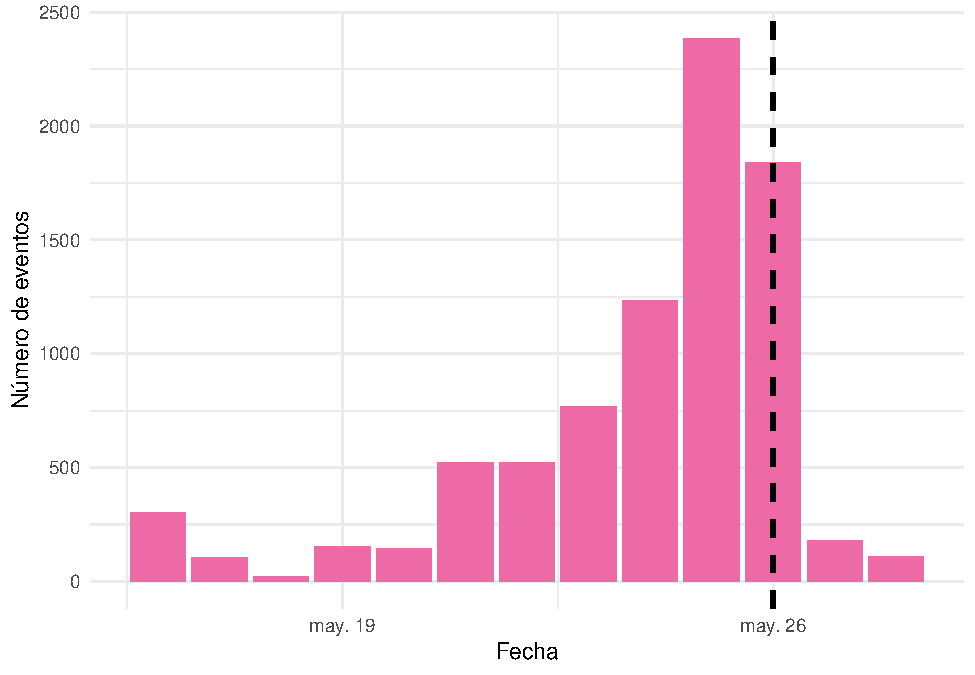
\includegraphics[width=1\linewidth]{ProyectoTD2026_files/figure-latex/picos-entrega-1} 

}

\caption{Actividad diaria en los días previos a la entrega final del proyecto (26 de mayo).}\label{fig:picos-entrega}
\end{figure}

En la Figura \ref{fig:picos-entrega} podemos identificar una evolución
creciente de la actividad a medida que se aproxima la fecha límite. El
mayor pico de actividad no se produce el mismo día de la entrega, sino
durante la jornada anterior, la cual se dedica a la depuración y
preparación del trabajo, limitándose el último día simplemente a
efectuar la entrega. Por tanto,los datos demuestran que el trabajo no se
planificó de forma escalonada, sino que más del 70\% del esfuerzo total
del periodo evaluado se condensó en las 24 horas inmediatamente
anteriores a la fecha límite.

\section{Exploración Usuarios}\label{exploraciuxf3n-usuarios}

En este apartado realizaremos un análisis en base al comportamiento de
los usuarios de la plataforma.

\subsection{Análisis frecuencia:usuarios más
activos}\label{anuxe1lisis-frecuenciausuarios-muxe1s-activos}

\begin{figure}

{\centering 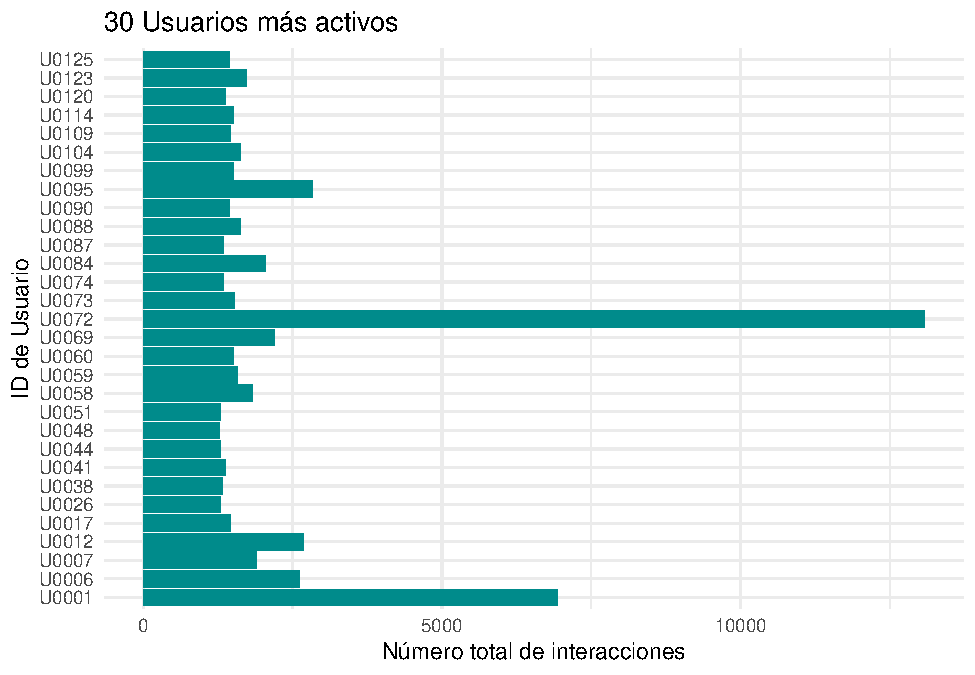
\includegraphics[width=1\linewidth]{ProyectoTD2026_files/figure-latex/grafico-usuarios-activos-1} 

}

\caption{30 usuarios con mayor número de interacciones en la plataforma.}\label{fig:grafico-usuarios-activos}
\end{figure}

Con el objetivo de analizar la participación por parte del alumnado,
hemos identificado los 30 usuarios más activos del conjunto.Como podemos
ver en la figura \ref{fig:grafico-usuarios-activos},existe un grupo de
alumnos con un número elevado de interacciones,llegando a ser más de
5000.

Este gráfico nos permite diferenciar el alumnado que utiliza la
plataforma de forma puntual y aquellos que navegan e interactúan
constantemente con el material del curso.

\subsection{Número medio de acciones por
usuario}\label{nuxfamero-medio-de-acciones-por-usuario}

\begin{Shaded}
\begin{Highlighting}[]
\NormalTok{acciones\_por\_usuario }\OtherTok{\textless{}{-}}\NormalTok{ datos\_logs }\SpecialCharTok{\%\textgreater{}\%}
  \FunctionTok{group\_by}\NormalTok{(Usuario) }\SpecialCharTok{\%\textgreater{}\%}
  \FunctionTok{summarise}\NormalTok{(}\AttributeTok{total\_acciones =} \FunctionTok{n}\NormalTok{(), }\AttributeTok{.groups =} \StringTok{"drop"}\NormalTok{) }\CommentTok{\# número total de acciones por cada usuario}
\NormalTok{media }\OtherTok{\textless{}{-}} \FunctionTok{mean}\NormalTok{(acciones\_por\_usuario}\SpecialCharTok{$}\NormalTok{total\_acciones)}
\end{Highlighting}
\end{Shaded}

Tras procesar los registros, se ha determinado que el número medio de
acciones realizadas por usuario es de 1261.448 Este dato sugiere que, en
promedio, cada estudiante interactúa más de 800 veces con la plataforma
a lo largo del periodo analizado, lo que refleja un seguimiento
constante de los materiales.

\subsection{Comportamientos atípicos}\label{comportamientos-atuxedpicos}

\begin{longtable}[t]{lr}
\caption{\label{tab:tabla-atipicos}Usuarios con comportamiento atípico en número de acciones}\\
\toprule
Usuario & total\_acciones\\
\midrule
U0072 & 13079\\
U0001 & 6932\\
U0095 & 2836\\
U0012 & 2680\\
U0006 & 2623\\
\bottomrule
\end{longtable}

Como se observa en la Tabla \ref{tab:tabla-atipicos} , existe un grupo
de estudiantes con una actividad excepcionalmente alta. Estos usuarios
suelen ser los que consultan repetidamente los materiales o realizan
múltiples intentos en las actividades, lo que debe tenerse en cuenta
para no sesgar las interpretaciones globales del grupo. Por ejemplo el
usuario U0072 destaca con un total de 13079 acciones, seguido por U0001
con 6932 acciones.

\section{Actividades}\label{actividades}

En este apartado veremos las diferentes relaciones, iteracciones y
comportamientos que tienen las actividades.

\subsection{Relación entre dispositivo empleado y la actividad
realizada}\label{relaciuxf3n-entre-dispositivo-empleado-y-la-actividad-realizada}

\begin{longtable}[t]{llr}
\caption{\label{tab:tabla-origen}Relación entre el origen y el tipo de evento}\\
\toprule
Origen & Evento & total\\
\midrule
web & Módulo de curso visto & 23535\\
web & Curso visto & 20430\\
cli & Usuario calificado & 340\\
web & Usuario calificado & 12506\\
web & Se ha visualizado el estado de la entrega. & 9388\\
\addlinespace
web & Intento de cuestionario visualizado & 3877\\
web & Intento de cuestionario actualizado & 3676\\
web & Pregunta creada & 3395\\
web & Informe de notas de usuario visto & 2771\\
web & Informe de sesión visto & 2680\\
\bottomrule
\end{longtable}

En la Tabla \ref{tab:tabla-origen} se aprecia cómo ciertos eventos de
consulta son predominantes desde determinados orígenes de conexión, lo
que sugiere que el tipo de dispositivo podría condicionar la navegación
del usuario. Por ejemplo el origen web con el tipo de evento Módulo de
curso visto con 23535.

\subsection{Actividades/recursos con más
iteracciones}\label{actividadesrecursos-con-muxe1s-iteracciones}

\begin{longtable}[t]{llr}
\caption{\label{tab:tabla-iteraccion2}Actividades o recursos con más interacciones}\\
\toprule
Componente & Evento & total\_interacciones\\
\midrule
Sistema & Curso visto & 20430\\
Tarea & Módulo de curso visto & 12860\\
Sistema & Usuario calificado & 12846\\
Tarea & Se ha visualizado el estado de la entrega. & 9388\\
Cuestionario & Intento de cuestionario visualizado & 3877\\
\addlinespace
Cuestionario & Intento de cuestionario actualizado & 3676\\
Sistema & Pregunta creada & 3395\\
Carpeta & Módulo de curso visto & 3310\\
Cuestionario & Módulo de curso visto & 3234\\
Usuario & Informe de notas de usuario visto & 2771\\
\bottomrule
\end{longtable}

Tal y como indica la Tabla \ref{tab:tabla-iteraccion2} , los componentes
relacionados con la visualización de materiales y la gestión de tareas
son los que generan el mayor flujo de datos en los logs analizados.

El componente sistema por ejemplo, con el evento curso visto con un
total de iteracciones 20430.

\section{Estudio de la actividad nocturna en periodos de
exámenes.}\label{estudio-de-la-actividad-nocturna-en-periodos-de-exuxe1menes.}

En este apartado analizaremos si existen accesos al Aula Virtual en
horarios poco habituales, el estudio se ha realizado con actividades
registradas entre las 00:00 y las 05:00 AM. Será posible analizar si
dichos accesos corresponden a casos aislados o, por el contrario,
aumentan durante periodos de evaluación.

\begin{Shaded}
\begin{Highlighting}[]
\NormalTok{Hora}\OtherTok{\textless{}{-}}\NormalTok{ datos\_logs }\SpecialCharTok{\%\textgreater{}\%}
  \FunctionTok{mutate}\NormalTok{(}
  \CommentTok{\# Extraemos la hora del df.}
  \AttributeTok{Hora\_dia=} \FunctionTok{hour}\NormalTok{(Fecha\_aux),}
  
  \CommentTok{\# Extraemos el día del df.}
  \AttributeTok{Fecha\_s=} \FunctionTok{as.Date}\NormalTok{(Fecha\_aux)}
\NormalTok{    ) }\SpecialCharTok{\%\textgreater{}\%}
  
  \CommentTok{\# Filtramos las horas consideradas "extrañas"}
  \FunctionTok{filter}\NormalTok{(Hora }\SpecialCharTok{\textgreater{}=} \DecValTok{0} \SpecialCharTok{\&}\NormalTok{ Hora }\SpecialCharTok{\textless{}=} \DecValTok{5}\NormalTok{) }\SpecialCharTok{\%\textgreater{}\%} 
  
  \CommentTok{\# Agrupamos por día}
  \FunctionTok{group\_by}\NormalTok{(Fecha\_s) }\SpecialCharTok{\%\textgreater{}\%} 
  
  \CommentTok{\#Calculamos el número de usuarios únicos}
  \FunctionTok{summarise}\NormalTok{(}\AttributeTok{Usuarios\_Unicos =} \FunctionTok{n\_distinct}\NormalTok{(Usuario))}
\end{Highlighting}
\end{Shaded}

\begin{figure}

{\centering 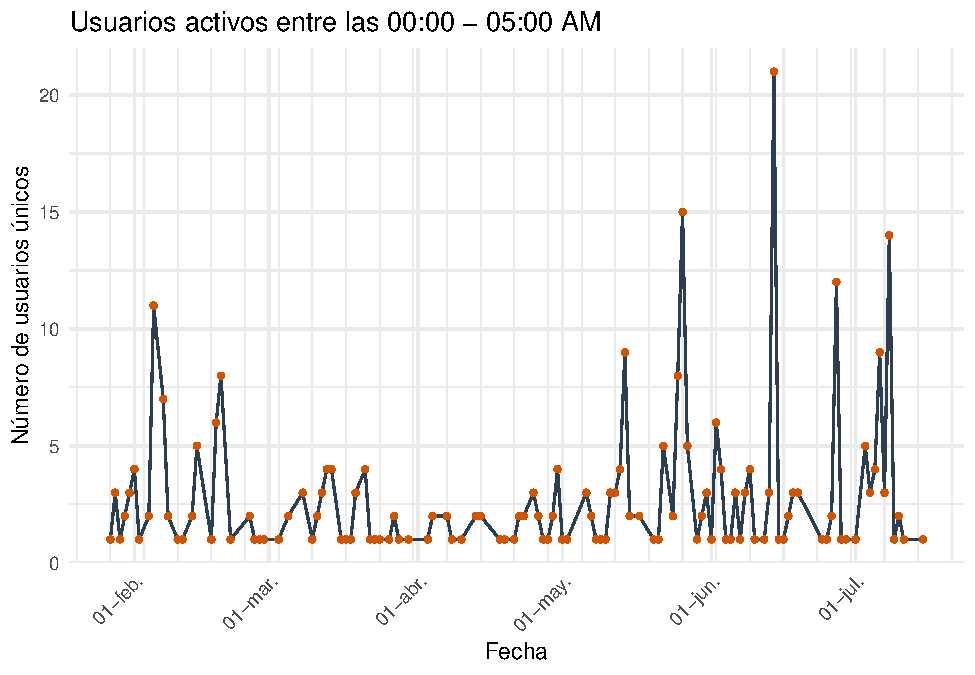
\includegraphics[width=1\linewidth]{ProyectoTD2026_files/figure-latex/grafico-usuarios-nocturnos-1} 

}

\caption{grafico usuarios nocturnos}\label{fig:grafico-usuarios-nocturnos}
\end{figure}

En el gráfico \ref{fig:grafico-usuarios-nocturnos} se observa que
durante el curso la actividad registrada en horario nocturno es
relativamente baja y corresponde mayoritariamente a usuarios aislados.

En el gráfico \ref{fig:grafico-usuarios-nocturnos} muestra la evolución
del segundo cuatrimestre en cuanto a la actividad de usuarios en horas
``extrañas'' (00:00 a 05:00 AM). Se observan claros picos de actividad
en algunos periodos del año, especialmente entre los meses de mayo y
julio. Mientras que durante el resto del curso la actividad es mínima y
podemos atribuirlo a usuarios aislados.

Sin embargo, conforme se aproximan los periodos de evaluación, el número
de estudiantes activos durante la madrugada aumenta de manera
considerable. Este comportamiento resulta especialmente visible entre
los meses de mayo y junio, coincidiendo la época de exámenes.

Con el objetivo de analizar con mayor detalle este periodo, se ha
generado una segunda visualización centrada únicamente en los meses de
mayo y julio.

\begin{figure}

{\centering 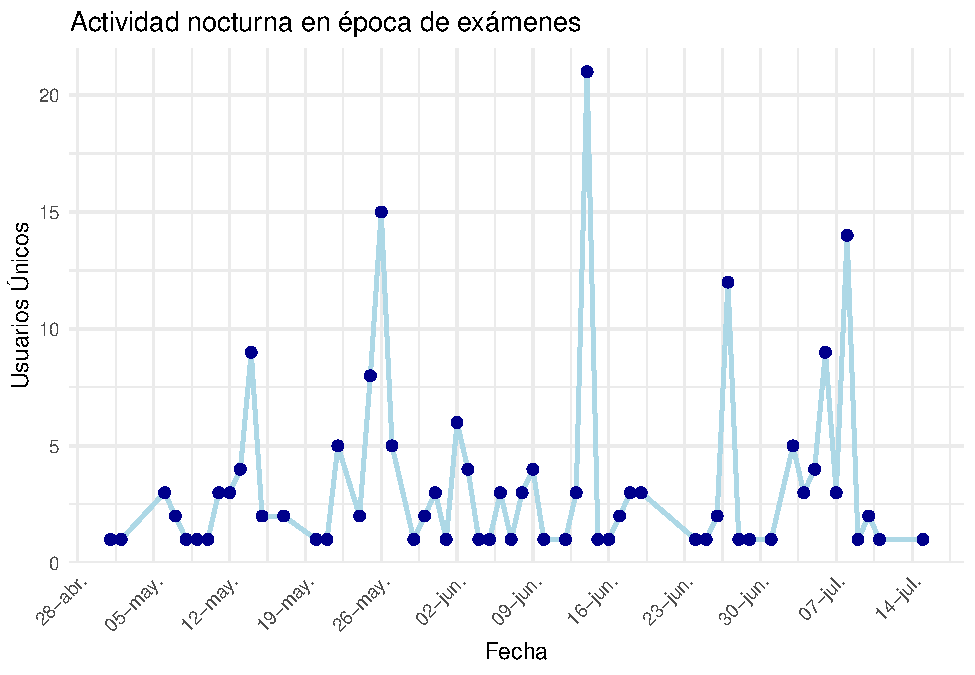
\includegraphics[width=1\linewidth]{ProyectoTD2026_files/figure-latex/grafico-epoca-examenes-1} 

}

\caption{epoca examenes}\label{fig:grafico-epoca-examenes}
\end{figure}

Como se aprecia en la Figura \ref{fig:grafico-epoca-examenes} , existen
varios días concretos donde la actividad nocturna aumenta notablemente.
Por ejemplo, alrededor del 26 de mayo y mediados de junio se registran
picos superiores a 15 y 20 usuarios conectados respectivamente durante
la madrugada.

Por otra parte, se puede ver casos aislados en algunos meses. Por
ejemplo entre el 5 de mayo y el 12 de mayo donde la actividad nocturna
se reduce a 1 o 2 usuarios por noche.

\section{Identificación de cambios de dirección IP en cortos periodos de
tiempo.}\label{identificaciuxf3n-de-cambios-de-direcciuxf3n-ip-en-cortos-periodos-de-tiempo.}

Se ha realizado un análisis para estudiar los posibles cambios de
conexión entre los usuarios mediantelas direcciones IP registradas en
los accesos del Aula Virtual. Este proceso perimite detectar si un mismo
usuario accede desde diferentes redes o dispositivos en intervalos
temporales reducidos.

\begin{longtable}[t]{lrr}
\caption{\label{tab:tabla-usuarios-ip-distinta}Usuarios con cambios frecuentes de IP}\\
\toprule
Usuario & IPs distintas totales & Cambios rápidos de IP\\
\midrule
U0001 & 1248 & 1167\\
U0006 & 153 & 48\\
U0003 & 112 & 39\\
U0102 & 123 & 35\\
U0012 & 73 & 33\\
\addlinespace
U0058 & 113 & 33\\
\bottomrule
\end{longtable}

Al analizar la Tabla \ref{tab:tabla-usuarios-ip-distinta}, se confirma
la existencia de accesos desde múltiples direcciones IP en intervalos de
tiempo muy reducidos. Destaca especialmente el usuario U0001, que
presenta un número muy elevado tanto de direcciones IP distintas como de
cambios rápidos de conexión (cada 30 minutos). Sin embargo, en la
mayoría de los usuarios los valores observados son considerablemente más
moderados.

Estos cambios tan frecuentes se deben a cambios de red (Wifi y datos
móviles), el uso de diferentes dispositivos o aquellas redes que son
dinámicas.

\section{Identificación de eventos de errores y acciones
fallidas.}\label{identificaciuxf3n-de-eventos-de-errores-y-acciones-fallidas.}

Para determinar si existen eventos de error o acciones fallidas
recurrentes en los logs del Aula Virtual, realizaremos un análisis de
aquellas acciones cuyo nombre contenga términos asociados a errores,
fallos o intentos no completados correctamente.

Este análisis puede resultar relevante ya que permite identificar los
posibles problemas técnicos o dificultades de uso de la plataforma del
Aula Virtual por parte de los usuarios.

\begin{Shaded}
\begin{Highlighting}[]
\CommentTok{\# Representamos gráficamente los eventos de error más frecuentes}
\FunctionTok{ggplot}\NormalTok{(eventos\_error, }\FunctionTok{aes}\NormalTok{(}\AttributeTok{x =} \FunctionTok{reorder}\NormalTok{(Evento, Total),}
           \AttributeTok{y =}\NormalTok{ Total)) }\SpecialCharTok{+}
  
  \CommentTok{\# Creamos las barras}
  \FunctionTok{geom\_col}\NormalTok{(}\AttributeTok{fill =} \StringTok{"cadetblue"}\NormalTok{) }\SpecialCharTok{+}
  
  
  \CommentTok{\# Añadimos las etiquetas con los valores}
  \FunctionTok{geom\_text}\NormalTok{(}\FunctionTok{aes}\NormalTok{(}\AttributeTok{label =}\NormalTok{ Total),}
            \AttributeTok{hjust =} \SpecialCharTok{{-}}\FloatTok{0.1}\NormalTok{,}
            \AttributeTok{size =} \FloatTok{3.5}\NormalTok{) }\SpecialCharTok{+}
  
  \CommentTok{\# Giramos el gráfico}
  \FunctionTok{coord\_flip}\NormalTok{() }\SpecialCharTok{+}
  
  \CommentTok{\# Añadimos títulos y etiquetas}
  \FunctionTok{labs}\NormalTok{(}
    \AttributeTok{title =} \StringTok{"Frecuencia de Eventos erróneos o Acciones fallidas"}\NormalTok{,}
    \AttributeTok{x =} \StringTok{"Tipo de evento"}\NormalTok{,}
    \AttributeTok{y =} \StringTok{"Número de registros"}\NormalTok{) }\SpecialCharTok{+}
  \FunctionTok{theme\_minimal}\NormalTok{()}
\end{Highlighting}
\end{Shaded}

\begin{figure}

{\centering 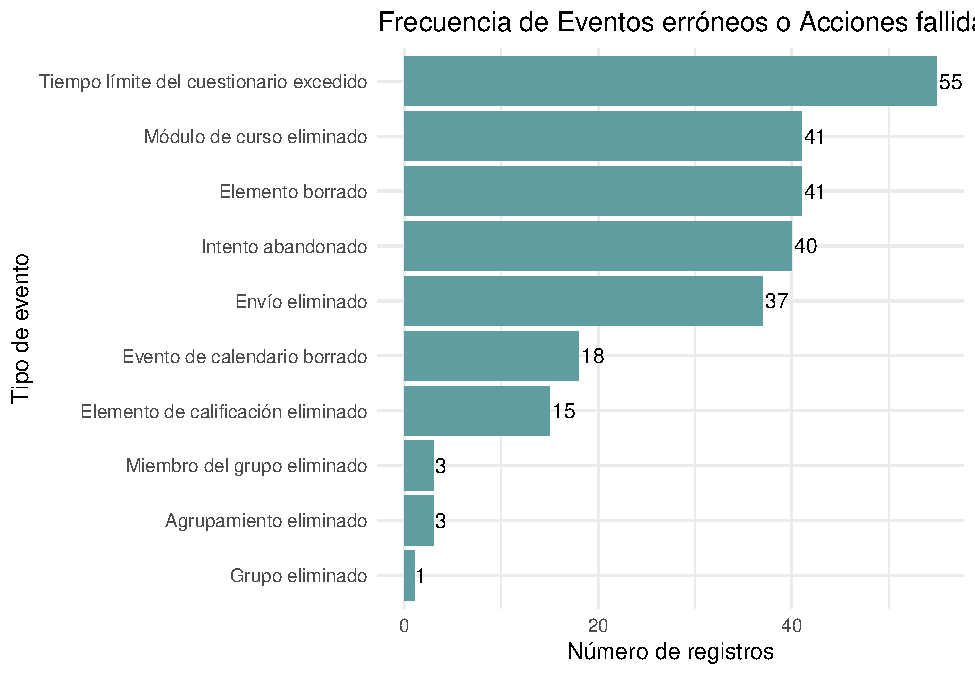
\includegraphics[width=1\linewidth]{ProyectoTD2026_files/figure-latex/grafico-eventos-erroneos-1} 

}

\caption{eventos de error más frecuentes.}\label{fig:grafico-eventos-erroneos}
\end{figure}

En el gráfico \ref{fig:grafico-eventos-erroneos} se pueden observar
aquellos eventos de errores o acciones fallidas que presentan una mayor
frecuencia dentro de los registros del Aula Virtual.

El evento más repetido corresponde a ``Tiempo límite del cuestionario
excedido'', con un total de 55 registros. También destacan los eventos
``Módulo de curso eliminado'' y ``Elemento borrado'', ambos con 41
registros.

Por otro lado, los eventos menos frecuentes son ``Grupo eliminado'' o
``Agrupamiento eliminado'' con un total de 3 y 1 registros
respectivamente. Esto puede indicar que son incidencias muy puntuales.

\subsection{Variación de la actividad anual en casos
aislados}\label{variaciuxf3n-de-la-actividad-anual-en-casos-aislados}

Para el análisis de la variación de la actividad de cada usuario a lo
largo del año, analizaremos las actividades registradas por cada usuario
en los diferentes meses y representaremos en un gráfico de barras los
datos de cada mes para poder observar la diferencia entre los meses.

\begin{figure}

{\centering 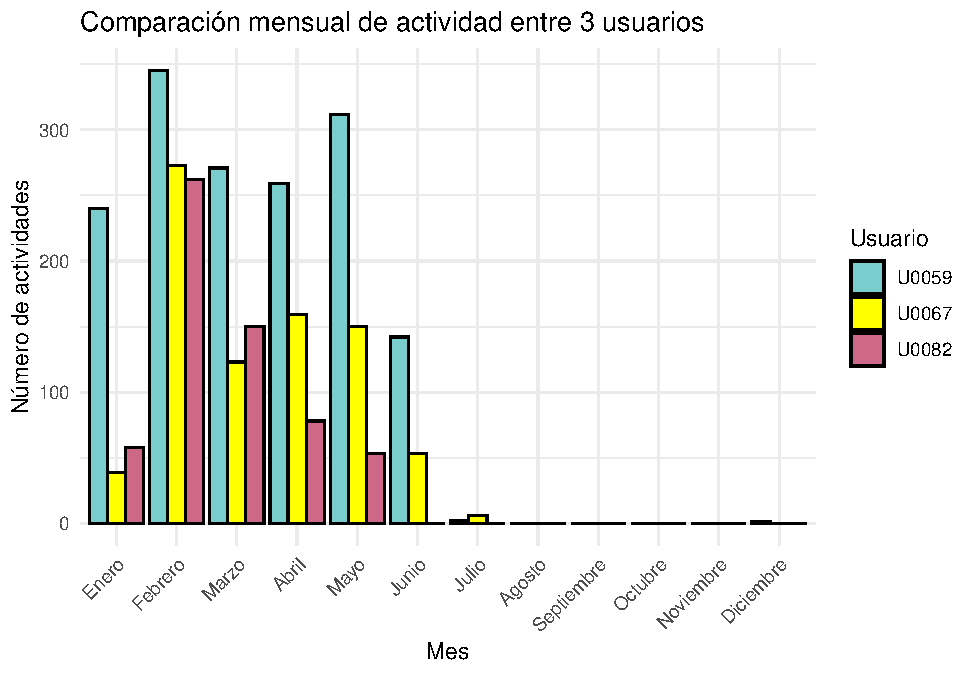
\includegraphics[width=1\linewidth]{ProyectoTD2026_files/figure-latex/graficos-actvidad-anual-1} 

}

\caption{variación actividad anual}\label{fig:graficos-actvidad-anual}
\end{figure}

Como observamos en el gráfico (\ref{fig:graficos-actvidad-anual}), cada
usuario presenta una variación anual de la actividad mensual diferente,
es decir que ninguno sigue un patrón organizado, ni los usuarios
muestran una misma variación entre los meses, por lo que según los datos
registrados podemos concluir en que cada usuario realiza una serie de
actividades diferentes independientemente de las actividades realizadas
por los demás usuarios del registro.

Por otra parte, algo que si podemos observar como ``normal'' en todos
los usuarios estudiados es la falta de actividad durante los meses de
agosto a diciembre, este suceso podemos suponer que no se sale de lo
previsto, puesto que sabemos de ante mano que se trata del registro de
las actividades realizadas en la asignatura de Tratamiento de Datos, la
cual se desarrolla durante el segundo cuatrimestre. Es por ello que no
es extraño que durante los meses del primer cuatrimestre, así como los
meses de verano, naturalmente, no presenten actividad alguna.

\subsection{Diferencias de actividad entre días lectivos y fines de
semana}\label{diferencias-de-actividad-entre-duxedas-lectivos-y-fines-de-semana}

Para analizar si existe una diferencia notable entre la actividad
registrada en días lectivos y la registrada durante los fines de semana,
estudiaremos el número total de eventos generados en cada día. El
objetivo es comprobar si los usuarios utilizan el aula virtual
principalmente durante la semana, coincidiendo con el calendario
académico, o si también muestran actividad relevante durante los sábados
y domingos. Para ello, clasificaremos cada registro según el día de la
semana y representaremos los resultados en un gráfico comparativo que
permita visualizar de forma clara la diferencia entre ambos grupos.

\textless\textless\textless\textless\textless\textless\textless{} HEAD

\begin{figure}

{\centering 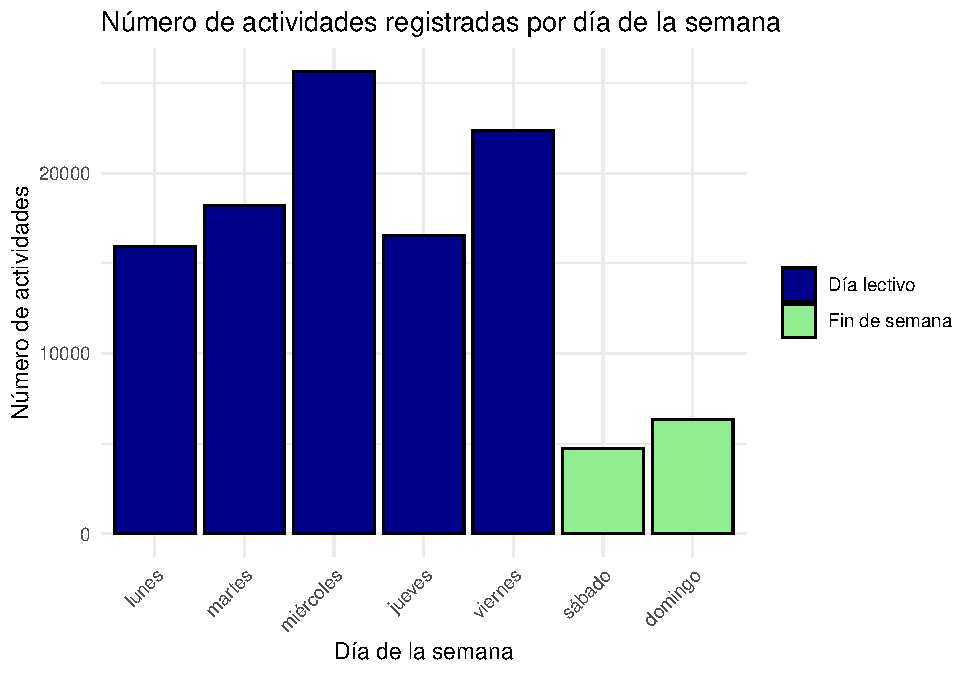
\includegraphics[width=1\linewidth]{ProyectoTD2026_files/figure-latex/dif_dias_fines-1} 

}

\caption{diferencia de actividad}\label{fig:dif_dias_fines}
\end{figure}

En el gráfico \ref{fig:dif_dias_fines} se observa la distribución de
actividades registradas a lo largo de los siete días de la semana. Los
días lectivos (de lunes a viernes) concentran la mayor parte de la
actividad, lo cual es coherente con el funcionamiento habitual de una
asignatura universitaria: los estudiantes suelen acceder al aula virtual
coincidiendo con las clases, la realización de tareas y la consulta de
materiales.

Por el contrario, los sábados y domingos muestran una actividad
considerablemente menor. Este descenso puede deberse a que los
estudiantes tienden a desconectar durante el fin de semana o a que la
asignatura no plantea entregas ni actividades en esos días. Además, si
se observa un pico concreto en algún día específico (por ejemplo, los
miércoles), podría estar relacionado con la programación de clases
presenciales, la publicación de materiales o la proximidad de fechas de
entrega.

En conjunto, el gráfico permite visualizar de forma clara cómo se
distribuye la actividad semanal y confirma que el uso de la plataforma
sigue un patrón muy ligado al calendario académico, los días lectivos se
registran actividades en mayor cantidad y los dias del fin de semana
menor.

\subsection{Variabilidad en la masa de estudiantes por
hora}\label{variabilidad-en-la-masa-de-estudiantes-por-hora}

Para analizar qué franjas horarias presentan una mayor variabilidad
entre usuarios, estudiaremos cuántos usuarios distintos generan
actividad en cada hora del día. Esto nos permitirá identificar si
existen horas en las que muchos usuarios diferentes acceden a la
plataforma, frente a otras en las que solo unos pocos usuarios realizan
acciones. Este análisis es útil para comprender los patrones colectivos
de acceso y detectar momentos de mayor diversidad de participación.

\textless\textless\textless\textless\textless\textless\textless{} HEAD

\begin{figure}

{\centering 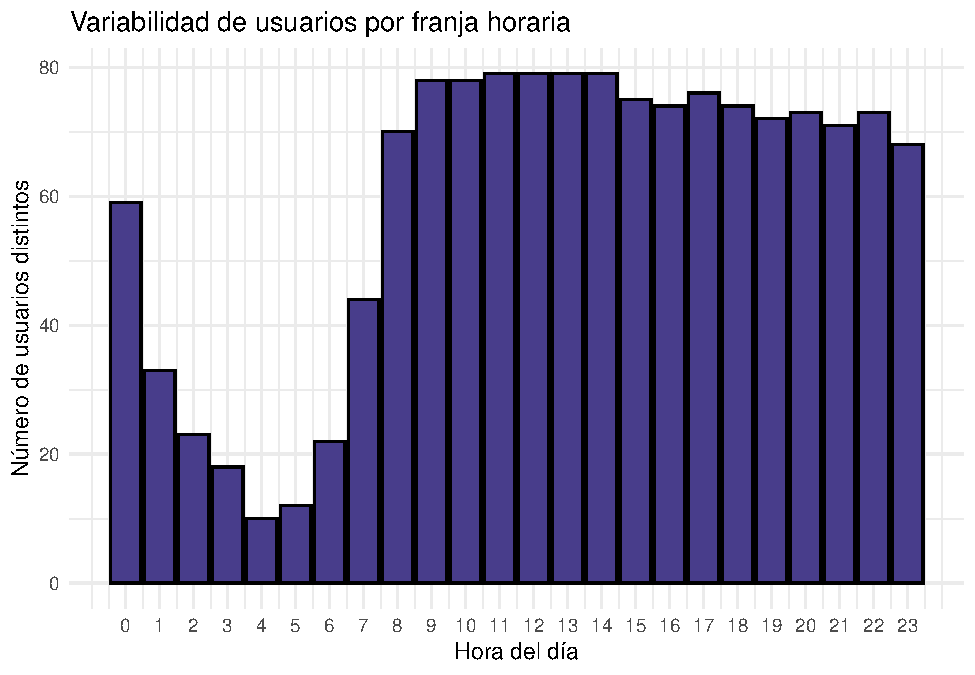
\includegraphics[width=1\linewidth]{ProyectoTD2026_files/figure-latex/grafico-variabilidad-1} 

}

\caption{variabilidad}\label{fig:grafico-variabilidad}
\end{figure}

El gráfico \ref{fig:grafico-variabilidad} muestra cuántos usuarios
distintos generan actividad en cada hora del día. Las horas con barras
más altas representan franjas horarias con mayor variabilidad, es decir,
momentos en los que muchos usuarios diferentes acceden a la plataforma.
Mientras que las barras más bajas muestran los momentos del día de menor
actividad por parte de los estudiantes.

Según lo que vemos en nuestro gráfico \ref{fig:grafico-variabilidad} ,
apartir de las 9am existe un número de usuarios muy superior a las horas
anteriores, vemos como este número continua estable durante las
siguientes horas hasta las 2pm, hora apartir de la cual comienza a
descender levemente, esto puede deberse a que apartir de las 9am y hasta
las 2pm los estudiantes se encuentran en horario lectivo, horarios con
clase, y vemos como la actividad sigue presente durante las horas de la
tarde, pero este número va decreciendo. En cambio, llegados ya a las
horas nocturas y durante las primeras horas de la mañana, vemos como esa
masa tan alta descience notoriamente, esto se debe, naturalmente a las
horas de descanso y sueño de los estudiantes.

En conjunto, el gráfico \ref{fig:grafico-variabilidad} permite
identificar claramente qué franjas horarias presentan mayor diversidad
de usuarios activos y cuáles muestran un uso más limitado,
proporcionando una visión global del comportamiento colectivo a lo largo
del día.

\subsection{Comportamiento del usuario: Actividades pasivas frente a
activas}\label{comportamiento-del-usuario-actividades-pasivas-frente-a-activas}

Para profundizar en la exploración de los usuarios, resulta fundamental
conocer qué tipo de uso hacen de la plataforma. Por ello, se procederá a
analizar la proporción existente entre el número de actividades pasivas
(orientadas a la consulta, como entrar o visualizar material) y las
actividades activas (que implican la creación o modificación de
contenido, como entregar tareas o editar).

Para dar respuesta a esta cuestión, se ha llevado a cabo una
clasificación de los eventos mediante técnicas de procesamiento de
texto. Se ha normalizado el texto y buscado raíces de palabras clave
para categorizar cada acción, otorgando prioridad a los eventos de
creación y excluyendo los eventos neutros o del sistema para asegurar
una comparativa directa y rigurosa.

\begin{longtable}[t]{lrr}
\caption{\label{tab:tabla-proporcion}Frecuencia y porcentaje de actividades Pasivas y Activas}\\
\toprule
Tipo\_Actividad & Cantidad & Porcentaje\\
\midrule
Activa & 28318 & 32.03\\
Pasiva & 60087 & 67.97\\
\bottomrule
\end{longtable}

Tal y como se muestra en la Tabla \ref{tab:tabla-proporcion}, existe una
evidente disparidad entre los volúmenes de ambas categorías. Para
facilitar la interpretación de estos resultados, se ha generado la
siguiente representación gráfica.

\begin{figure}[H]

{\centering 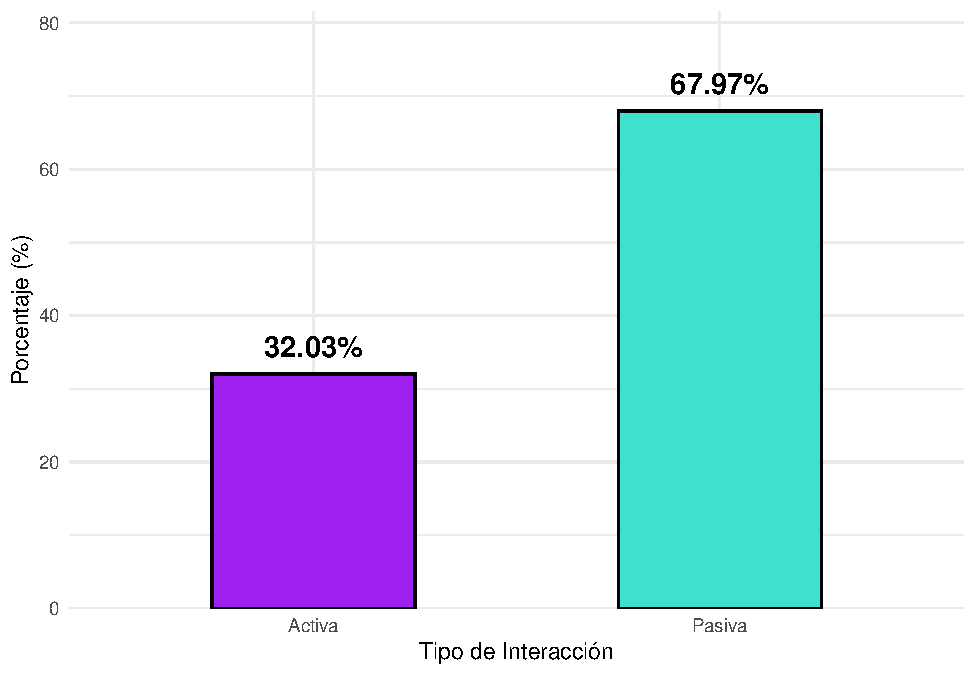
\includegraphics[width=1\linewidth]{ProyectoTD2026_files/figure-latex/figura-proporcion-1} 

}

\caption{Proporción de actividades pasivas frente a activas en la plataforma.}\label{fig:figura-proporcion}
\end{figure}

Como se observa en la Figura \ref{fig:figura-proporcion}, la diferencia
de comportamiento es muy notoria. La inmensa mayoría de las
interacciones registradas en el Aula Virtual consisten en el consumo
pasivo de contenido (visualización de cursos, descarga de apuntes o
lectura de enunciados). Las interacciones activas representan una
pequeña fracción del total, este es un patrón esperado en entornos de
aprendizaje virtual donde el estudio autónomo y la lectura preceden a
los momentos puntuales de entrega o evaluación.

\subsection{Identificación de patrones de acceso
estacional}\label{identificaciuxf3n-de-patrones-de-acceso-estacional}

Tras analizar la distribución general de la actividad, resulta de gran
interés determinar si existe un perfil de estudiante con un
comportamiento ``estacional''. Es decir, alumnos que no mantienen una
interacción constante con el Aula Virtual, sino que concentran gran
parte de su actividad en momentos críticos, como los días previos a la
entrega final del proyecto (fijada el 26 de mayo).

Para este análisis, hemos definido un ``Periodo Crítico'' que abarca los
7 días previos a la entrega. Hemos clasificado a los usuarios en dos
categorías: \textbf{Acceso Puntual}, aquellos cuya actividad semanal
triplica la media esperada (concentrando más del 10\% de sus clics
anuales en esa única semana); y \textbf{Acceso Regular}, el resto de
usuarios con una participación más constante a lo largo del curso.

\begin{longtable}[t]{lrr}
\caption{\label{tab:tabla-estacionalidad}\label{tab:tabla-estacional}Clasificación de usuarios según su estacionalidad ante la entrega.}\\
\toprule
Tipo\_Usuario & Numero\_Usuarios & Porcentaje\\
\midrule
Acceso Puntual & 21 & 24.14\\
Acceso Regular & 66 & 75.86\\
\bottomrule
\end{longtable}

Como se puede observar en la Tabla \ref{tab:tabla-estacional}, al
aplicar este criterio de concentración semanal, logramos identificar un
segmento de la clase con un perfil de acceso puntual. Aunque un gran
grupo de estudiantes mantiene una interacción más regular a lo largo del
curso, existe una parte del alumnado que intensifica drásticamente su
huella digital ante la proximidad de los plazos de evaluación.

Para visualizar esta segmentación y entender cómo se distribuye la
intensidad de la actividad en el periodo crítico, se presenta la
siguiente figura.

\begin{figure}[H]

{\centering 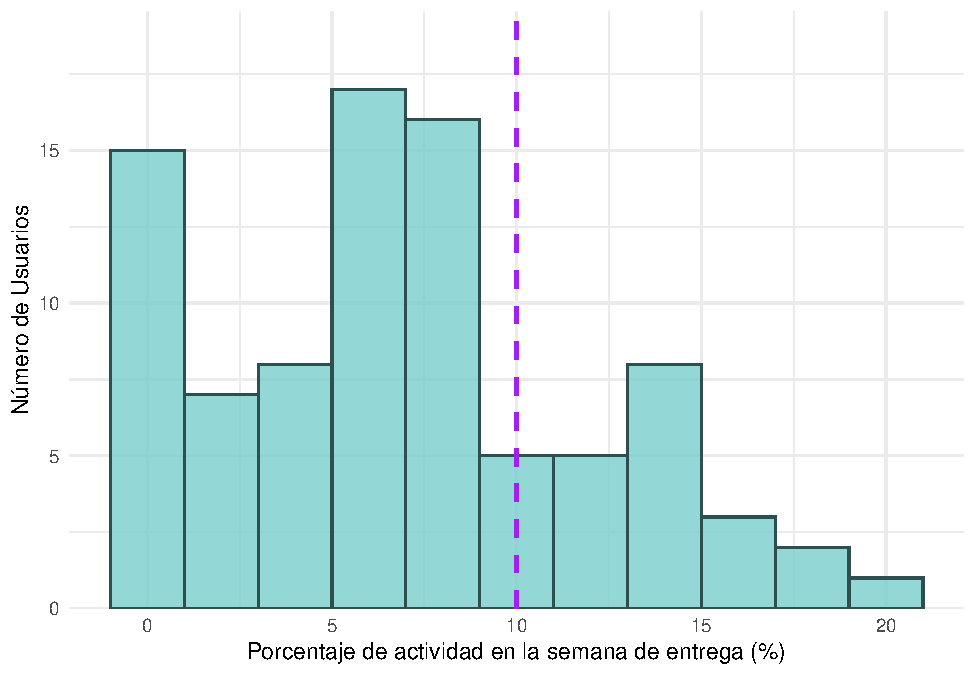
\includegraphics[width=1\linewidth]{ProyectoTD2026_files/figure-latex/figura-estacional-1} 

}

\caption{Concentración de la actividad de los usuarios en la plataforma durante periodos muy concretos.}\label{fig:figura-estacional}
\end{figure}

La Figura \ref{fig:figura-estacional} muestra la distribución de los
usuarios según el peso que tiene esa semana específica en su actividad
total anual. La acumulación de usuarios a la derecha de la línea de
corte (marcada en color morado) confirma la existencia de alumnos cuya
actividad se dispara bajo la presión evaluativa. Este comportamiento es
un indicador claro de una estrategia de aprendizaje basada en la
urgencia frente a la constancia continuada.

\subsection{Análisis del uso de dispositivos según la franja
horaria}\label{anuxe1lisis-del-uso-de-dispositivos-seguxfan-la-franja-horaria}

Para comprender los hábitos de conexión del alumnado, la cuestión
plantea si existe una disminución del uso de dispositivos móviles
durante el horario lectivo en favor de otras herramientas. Para
estructurar la comparativa, definimos el ``Horario Lectivo'' como la
franja comprendida entre las 08:00 y las 14:00 horas, frente al
``Horario No Lectivo'' (el resto del día).

Mediante funciones de búsqueda y filtrado de texto, rastreamos los
registros en busca de las etiquetas asociadas a la aplicación móvil
(App, Web Services, Mobile,\ldots) para contrastarlos con los accesos al
entorno web estándar.

\begin{longtable}[t]{llrr}
\caption{\label{tab:tabla-dispositivos}Distribución absoluta y porcentual del tipo de acceso por franja horaria.}\\
\toprule
Horario & Dispositivo & Accesos & Porcentaje\\
\midrule
Horario Lectivo & Ordenador / Web & 70765 & 100\\
Horario No Lectivo & Ordenador / Web & 38981 & 100\\
\bottomrule
\end{longtable}

Como se detalla en la Tabla \ref{tab:tabla-dispositivos}, los resultados
extraídos del conjunto de datos son tajantes y revelan una limitación
técnica de los propios registros de la plataforma: no existen trazas de
actividad móvil. El 100\% de las interacciones, tanto por la mañana como
por la tarde, constan en el sistema como tráfico Web/Ordenador.

Ante la imposibilidad de comparar porcentajes de dispositivos (dado que
la variable es constante), el análisis debe centrarse en el volumen
total de actividad que soporta la plataforma en cada una de estas
franjas.

\begin{verbatim}
## Warning in prettyNum(.Internal(format(x, trim, digits, nsmall, width, 3L, :
## 'big.mark' y 'decimal.mark' son ambos '.', lo cual puede ser confuso
\end{verbatim}

\begin{figure}[H]

{\centering 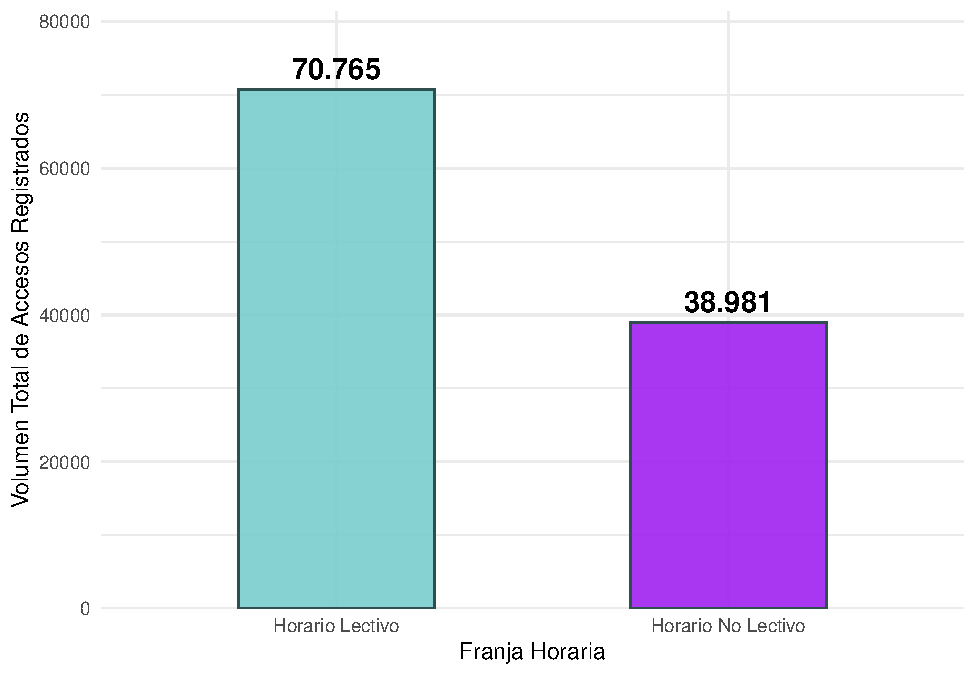
\includegraphics[width=1\linewidth]{ProyectoTD2026_files/figure-latex/figura-dispositivos-1} 

}

\caption{Actividad total en el Aula Virtual por franja horaria.}\label{fig:figura-dispositivos}
\end{figure}

A la vista de la Tabla \ref{tab:tabla-dispositivos} y la Figura
\ref{fig:figura-dispositivos}, se puede dar una respuesta fundamentada a
la pregunta de investigación planteada: el uso de dispositivos es
completamente indiferente respecto al horario. En la base de datos
analizada, el alumno utiliza invariablemente el entorno Web/Ordenador.

Lo que sí experimenta una variación altamente significativa no es la
herramienta, sino la intensidad de uso. La Figura
\ref{fig:figura-dispositivos} evidencia que el volumen de interacciones
se desploma casi a la mitad (pasando de más de 70.000 a cerca de 39.000)
al salir del horario de clase. Esto permite concluir que, aunque el
dispositivo no cambia, los estudiantes concentran su actividad digital
en la franja matutina presencial, dejando el horario no lectivo para un
acceso considerablemente más residual.

\subsection{Análisis de la actividad según el tipo de día y momento del
curso}\label{anuxe1lisis-de-la-actividad-seguxfan-el-tipo-de-duxeda-y-momento-del-curso}

Para comprender los hábitos de estudio del alumnado, es fundamental
analizar cómo se distribuye su carga de trabajo entre los días laborales
y los fines de semana. Además, resulta de gran interés comprobar si esta
proporción se mantiene estable a lo largo del año o si, por el
contrario, se ve alterada ante la proximidad de fechas clave (como la
entrega de proyectos o exámenes).

Para responder a esta cuestión, utilizamos la información temporal de
los eventos para identificar el día exacto de la semana en que
ocurrieron. Posteriormente, dividimos el histórico del curso en dos
fases: un Periodo Regular y una Época de Entrega (definida como los 14
días previos a la entrega final del proyecto fijada el 26 de mayo).

\begin{longtable}[t]{llrr}
\caption{\label{tab:tabla-dias}Distribución de la actividad en días laborales y fines de semana según la fase del curso.}\\
\toprule
Fase\_Curso & Tipo\_Dia & Accesos & Porcentaje\\
\midrule
Periodo Regular & Fin de Semana (S-D) & 7321 & 7.66\\
Periodo Regular & Laboral (L-V) & 88232 & 92.34\\
Época de Entrega & Fin de Semana (S-D) & 3746 & 26.39\\
Época de Entrega & Laboral (L-V) & 10447 & 73.61\\
\bottomrule
\end{longtable}

Al analizar la Tabla \ref{tab:tabla-dias}, debemos tener en cuenta un
factor estadístico clave: una semana se compone de 5 días laborales y 2
de fin de semana. Por tanto, un reparto equitativo y perfectamente
proporcional del trabajo implicaría, de base, un \textasciitilde71\% de
actividad laboral y un \textasciitilde29\% en fin de semana.

Para interpretar correctamente cómo los estudiantes alteran este balance
natural según el momento del curso, se ha diseñado la siguiente
visualización comparativa.

\textless\textless\textless\textless\textless\textless\textless{} HEAD

\begin{figure}[H]

{\centering 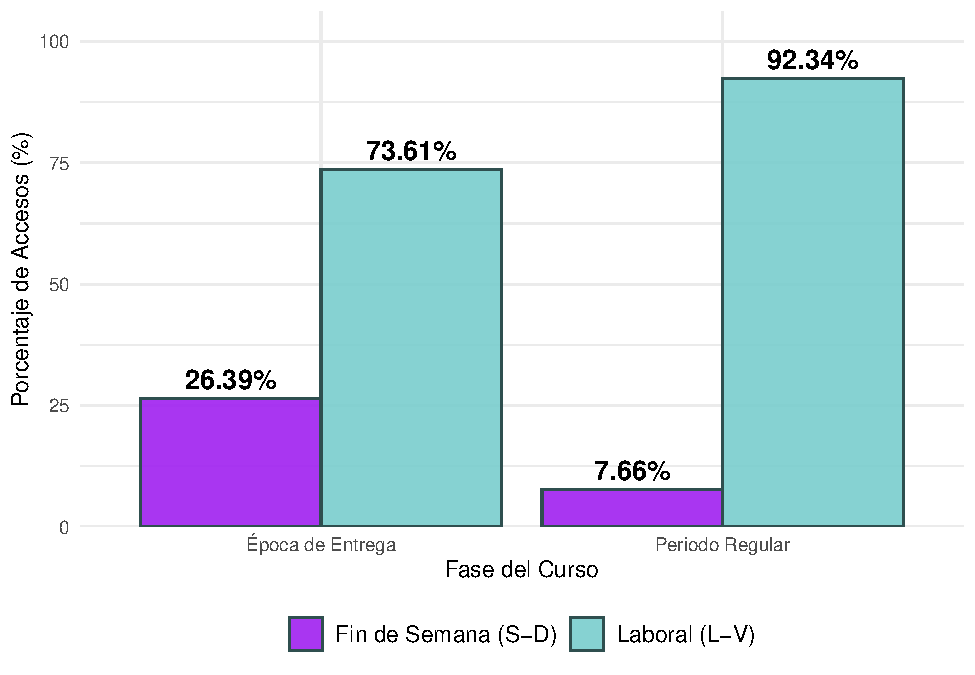
\includegraphics[width=1\linewidth]{ProyectoTD2026_files/figure-latex/figura-dias-1} 

}

\caption{Comparativa porcentual de accesos entre días laborales y fines de semana.}\label{fig:figura-dias}
\end{figure}

La Figura \ref{fig:figura-dias} responde claramente a la hipótesis
planteada. De forma general, existe mucha más actividad durante los días
laborales, algo lógico al ser los días en los que se imparte docencia y
los estudiantes asisten al campus. Durante el ``Periodo Regular'', el
fin de semana registra una actividad residual, evidenciando que el
alumnado utiliza estos días principalmente para el descanso y la
desconexión académica.

Sin embargo, esta proporción varía drásticamente al analizar momentos
concretos. Al llegar la ``Época de Entrega'', la gráfica muestra un
notable trasvase porcentual: el peso del fin de semana (representado por
las barras en color morado) se incrementa considerablemente a costa de
la actividad entre semana. Este aumento demuestra que, bajo la presión
de los plazos de evaluación o exámenes, los estudiantes se ven obligados
a sacrificar sus días de descanso y convertir los fines de semana en
jornadas intensivas de estudio y trabajo en la plataforma.

%%%%%%%%%%%%%%%%%%%%%%%%%%%%%%%%%%%%%%%%%%

\vspace{6pt}

%%%%%%%%%%%%%%%%%%%%%%%%%%%%%%%%%%%%%%%%%%
%% optional

% Only for the journal Methods and Protocols:
% If you wish to submit a video article, please do so with any other supplementary material.
% \supplementary{The following supporting information can be downloaded at: \linksupplementary{s1}, Figure S1: title; Table S1: title; Video S1: title. A supporting video article is available at doi: link.}

%%%%%%%%%%%%%%%%%%%%%%%%%%%%%%%%%%%%%%%%%%







%%%%%%%%%%%%%%%%%%%%%%%%%%%%%%%%%%%%%%%%%%
%% Optional

%% Only for journal Encyclopedia


%%%%%%%%%%%%%%%%%%%%%%%%%%%%%%%%%%%%%%%%%%
%% Optional
%%%%%%%%%%%%%%%%%%%%%%%%%%%%%%%%%%%%%%%%%%
\begin{adjustwidth}{-\extralength}{0cm}

%\printendnotes[custom] % Un-comment to print a list of endnotes



% If authors have biography, please use the format below
%\section*{Short Biography of Authors}
%\bio
%{\raisebox{-0.35cm}{\includegraphics[width=3.5cm,height=5.3cm,clip,keepaspectratio]{Definitions/author1.pdf}}}
%{\textbf{Firstname Lastname} Biography of first author}
%
%\bio
%{\raisebox{-0.35cm}{\includegraphics[width=3.5cm,height=5.3cm,clip,keepaspectratio]{Definitions/author2.jpg}}}
%{\textbf{Firstname Lastname} Biography of second author}

%%%%%%%%%%%%%%%%%%%%%%%%%%%%%%%%%%%%%%%%%%
%% for journal Sci
%\reviewreports{\\
%Reviewer 1 comments and authors’ response\\
%Reviewer 2 comments and authors’ response\\
%Reviewer 3 comments and authors’ response
%}
%%%%%%%%%%%%%%%%%%%%%%%%%%%%%%%%%%%%%%%%%%
\PublishersNote{}
\end{adjustwidth}


\end{document}
